\documentclass[11pt,a4paper]{ivoa}
\input tthdefs

\usepackage{array}
\usepackage{tabulary}  % for nicer tables
\usepackage{calc}
\usepackage{placeins}
\setlength\extrarowheight{2pt}

\newcolumntype{L}{>{\centering\arraybackslash}m{3cm}}

\title{Model Instances in Votables}

% see ivoatexDoc for what group names to use here
\ivoagroup{DM}

\newcommand{\TODO}[1]{%
    \noindent%
    \colorbox{todocolor}{%
            \parbox{0.85\linewidth}{\sffamily \textbf{TODO:}\\
            #1}
    }%
    \vspace{2pt}
}

\newcommand{\note}[1]{%
    \noindent%
    \textcolor{darkgrey}{{\sffamily Note:} \emph{#1}}%
}

\newcommand{\comment}[1]{%
    \noindent%
    \textcolor{red}{{\sffamily Comment:} \emph{#1}}%
}

%%%%%%%%%%%%%%%%%%%%%%%%%%%%%%%%%%%%
% XML syntax coloration and formatting
%
\definecolor{todocolor}{rgb}{1,1,0.8}
\definecolor{darkred}{rgb}{0.6,0,0}
\definecolor{rose}{rgb}{1.0,0.88,0.88}
\definecolor{darkgrey}{rgb}{0.35,0.35,0.35}
\definecolor{gray}{rgb}{0.4,0.4,0.4}
\definecolor{darkblue}{rgb}{0.0,0.0,0.6}
\definecolor{maroon}{rgb}{0.5,0,0}
\definecolor{cyan}{rgb}{0.0,0.6,0.6}

\lstset{
  basicstyle=\ttfamily,
  columns=fullflexible,
  showstringspaces=false,
  commentstyle=\color{gray}\upshape
}

\lstdefinelanguage{XML}
{
  morestring=[b]",
  morestring=[s]{>}{<},
  morecomment=[s]{<?}{?>}, 
  morecomment=[s]{<!--}{-->},
  stringstyle=\color{black},
  identifierstyle=\color{darkblue},
  keywordstyle=\color{maroon},
  morekeywords={ref,utype,dmrole, dmtype, value}% list your attributes here
}

\lstdefinestyle{XML}{
    captionpos=b,
    basicstyle=\small\ttfamily
}

%%%%%%%%%%%%%%%%%%%%%%%%%%%
% Document core
%
\author{François Bonnarel}
\author{Gilles Landais}
\author{Laurent Michel}
\author{Jesus Salgado}

\editor{Laurent Michel}

% \previousversion[????URL????]{????Concise Document Label????}
\previousversion{This is the first public release}
       

\begin{document}

\begin{abstract}
Vodml-instance-vot proposes a syntax to map VOTable data on any model serialized in VO-DML.
Vodml-instance-vot annotations are grouped in a single XML block located in the VOTable head. The annotation block allows to easily reconstruct the model structure. It designed in a way that the block can be reused on different data sets in order to facilitate the annotation process.
Vodml-instance-vot is enable to join data from different tables
\end{abstract}


\section*{Acknowledgments}
CDS/TDIG/SourceDM contributors

\section*{Conformance-related definitions}

The words ``MUST'', ``SHALL'', ``SHOULD'', ``MAY'', ``RECOMMENDED'', and
``OPTIONAL'' (in upper or lower case) used in this document are to be
interpreted as described in IETF standard RFC2119 \citep{std:RFC2119}.

The \emph{Virtual Observatory (VO)} is a
general term for a collection of federated resources that can be used
to conduct astronomical research, education, and outreach.
The \href{http://www.ivoa.net}{International
Virtual Observatory Alliance (IVOA)} is a global
collaboration of separately funded projects to develop standards and
infrastructure that enable VO applications.


\section{Introduction}



\lstset{language=XML}

\subsection{Role within the VO Architecture}

\begin{figure}
\centering

% As of ivoatex 1.2, the architecture diagram is generated by ivoatex in
% SVG; copy ivoatex/archdiag-full.xml to archdiag.xml and throw out
% all lines not relevant to your standard.
% Notes don't generally need this.  If you don't copy archdiag.xml,
% you must remove archdiag.svg from FIGURES in the Makefile.

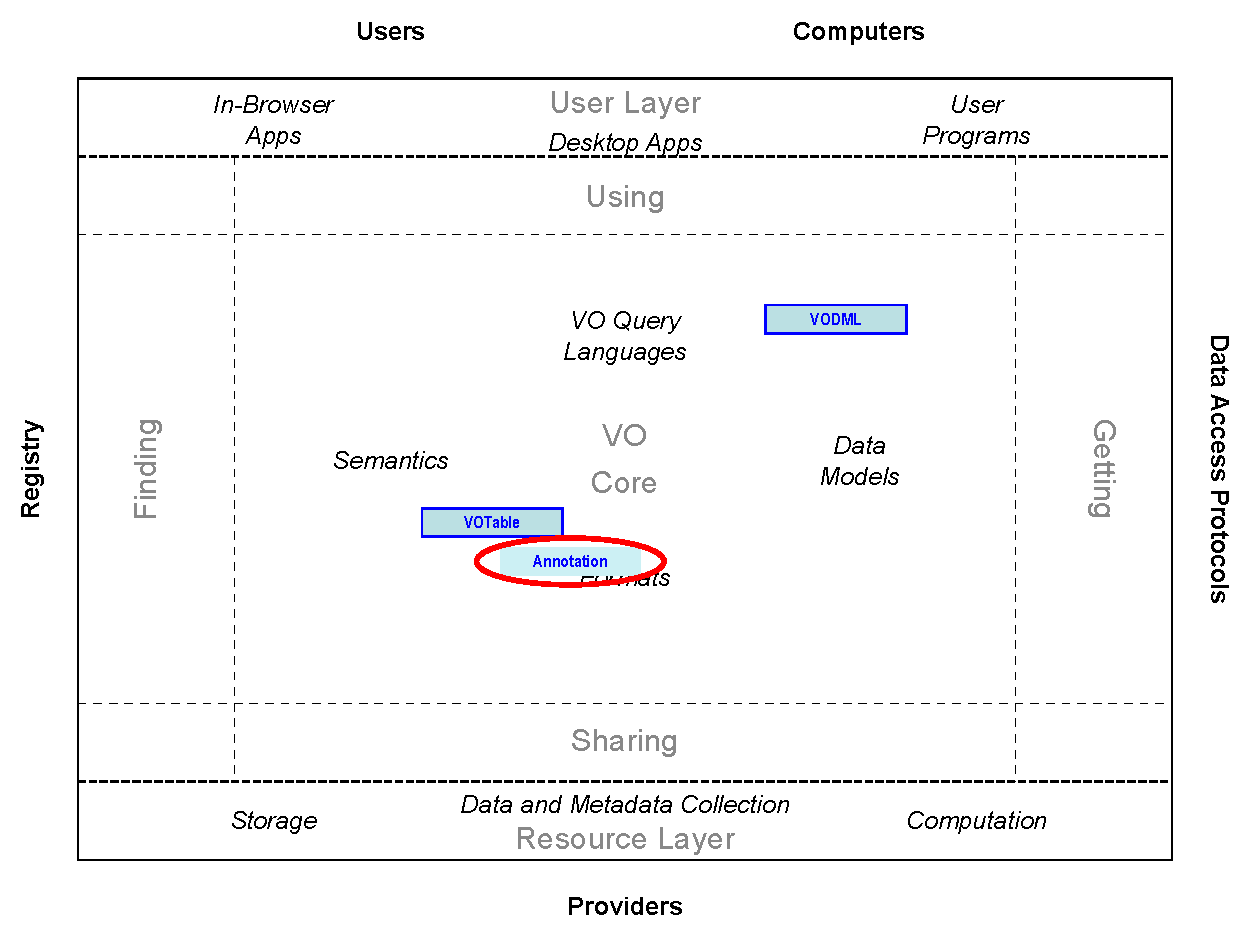
\includegraphics[width=0.9\textwidth]{role_diagram.pdf}
\caption{Architecture diagram for this document}
\label{fig:archdiag}
\end{figure}

Fig.~\ref{fig:archdiag} shows the role this document plays within the
IVOA architecture \citep{note:VOARCH}.

???? and so on, LaTeX as you know and love it. ????

\section{Use Cases and Requirement}

\subsection{Use Cases}




\section{Syntax}


The syntax rules specified in this standard allow to build consistent annotations for any model. However, they do not prevent to do foolish things in the same way that a programming language grammar does not protect people against writing irrelevant software.
In the following annotation snippets, the values of the XML elements attribute do not refer to any particular model or VOTable. They have been choosen to help readers to figure out their meanings.

\subsection{Mapping Block Structure}

The mapping block must be the first child of \texttt{VOTABLE}. Its scope is the whole VOTable. Its stucture is given below.

\begin{lstlisting}[caption={Complete mapping block example},style=XML]
<VOTABLE xmlns="http://www.ivoa.net/xml/VOTable/v1.3" 
            xmlns:xsi="http://www.w3.org/2001/XMLSchema-instance" 
            version="1.4">
   <MODEL_INSTANCE name="MANGO" 
              syntax="model-instance-in-vot"  
             uri="http://server.mango.vo-dml.xml">
     <GLOBALS>   ...  </GLOBALS>

      <TABLE\_MAPPING tableref=...>  ... </TABLE\_MAPPING tableref=...>
      <TABLE\_MAPPING tableref=...> ...  </TABLE\_MAPPING tableref=...>
    ...
   </MODEL_INSTANCE>
   ..
</VOTABLE>
\end{lstlisting}

The mapping construction rules are independant from any model or data layout either.

\begin{itemize}
    \item The mapping is located in a \texttt{<MODEL\_INSTANCE>} block, child of \texttt{<VOTABLE>}.
    \item The mapping elements denote the model structure.
    \item The first child of \texttt{<MODEL\_INSTANCE>} must be the \texttt{<GLOBALS>} block containing data shared by the whole mapping.    
    \item The \texttt{<GLOBALS>} block is followed a sequence of \texttt{<TABLE\_MAPPING>}.
    \item There is one \texttt{<TABLE\_MAPPING>} per mapped \texttt{<TABLE>}.
\end{itemize}
\FloatBarrier

%%%%%%%%%%%%%%%%%%%%%%%%%%%%%%%%%%%%%
%
% TOP LEVEL STRUCTURE
%
%%%%%%%%%%%%%%%%%%%%%%%%%%%%%%%%%%%%%

\subsection{Mapping Top Level Structure}
%%%%%%%%%%%%%%%%%%%%%%%%%%%%%%%%%%%%%
%
% MODELS
%

\subsubsection{MODEL\_INSTANCE}

The  \texttt{MODEL\_INSTANCE}  element encompasses the mapping block. 
This element can refer or not to a specific model. There no obligation to have a tight coupling between a mapping block and a specific model. The use of the model referenced  \texttt{MODEL\_INSTANCE}  is left at the discretion of the client. The client can just look for interesting quantities without regards on a particular model or on the opposite build a model instance by merging the vo-dml model serialization which URL is given here, with the mapping block.

\begin{table}[!htbp]
\small
\centering
\begin{tabulary}{\linewidth}{|c|J|}       
       \hline 
            \textbf{Attribute} & 
            \textbf {Role}\\
       \hline         \hline  
            @name  & 
            Name of the mapped model (informal).  This attribute must be left empty  \\
       \hline 
            @syntax  & 
            Syntax used for the mapping. The default syntax  is this proposed in this document\texttt{@syntax=model-instance-in-vot} . This attribute must be left empty when present.\\
       \hline 
            @uri  & 
            Uri of the vo-dml serialization of the mapped model. \\
       \hline 
     \end{tabulary}
     \caption{\texttt{MODEL\_INSTANCE} attributes} 
     \label{tbl:model-att}
 \end{table}

\begin{table}[!htbp]
\small
\centering
\begin{tabulary}{\linewidth}{|c|c|c|J|}
    \hline 
        \textbf{@name} &        
        \textbf{@syntax} &       
        \textbf{@uri} &
        \textbf{Pattern}\\
    \hline      \hline  
        MAND &           
        OPT &           
        OPT &   
        Always mandatory\\
   \hline 
\end{tabulary}
     \caption{Valid attribute patterns for  \texttt{MODEL\_INSTANCE}} 
     \label{tbl:model-pattern}
 \end{table}
\FloatBarrier

 \FloatBarrier

%%%%%%%%%%%%%%%%%%%%%%%%%%%%%%%%%%%%%
%
% GLOBALS
%

\subsubsection{GLOBALS}
 Contains  \texttt{INSTANCE}s  that can be used everywhere in the \texttt{MODEL\_INSTANCE}.

\begin{itemize}
    \item \texttt{INSTANCE}s children of \texttt{GLOBALS} should have an  \texttt{@ID} attribute so that they can be referenced from other instances.
    \item The role of the \texttt{GLOBALS}s children, (\texttt{INSTANCE}s by construction), must be ignored although being mandatory.
    \item References within \texttt{GLOBALS}s  sub-elements to VOTable data (\texttt{FIELD} ot \texttt{PARAM}) must be searched in all tables. 
            They must be resolved by the first occurence matching the reference found.
    \item \texttt{GLOBALS} has no attributes. 
\end{itemize}

\begin{lstlisting}[caption={GLOBALS block example},style=XML]
  <GLOBALS>
    <INSTANCE ID="SpaceCoordFrame" >
      <INSTANCE dmrole="coords:SpaceFrame.refPosition" 
                 dmtype="coords:StdRefLocation">
          <ATTRIBUTE dmrole="coords:StdRefLocation.position" 
                      dmtype="ivoa:string" value="NoSet"/>
      </INSTANCE>
      <ATTRIBUTE dmrole="coords:SpaceFrame.spaceRefFrame" 
                  dmtype="ivoa:string" value="ICRS"/>
      <ATTRIBUTE dmrole="coords:SpaceFrame.equinox" 
                  dmtype="coords:Epoch"   value="NoSet"/>
    </INSTANCE>
 </GLOBALS>
\end{lstlisting}




\begin{table}[!htbp]
\small
\centering
\begin{tabulary}{\linewidth}{|c|J|}       
       \hline 
           \textbf{Child} &  
           \textbf{Role}\\
       \hline         \hline  
            \texttt{INSTANCE}    &  
            Model instances with a scope covering the whole VOTable . \\       
       \hline 
     \end{tabulary}
     \caption{Allowed  \texttt{GLOBALS} children} 
     \label{tbl:globals-children}
 \end{table}

\FloatBarrier
%%%%%%%%%%%%%%%%%%%%%%%%%%%%%%%%%%%%%
%
% TABLE\MAPPING
%

\subsubsection{TABLE\_MAPPING}

\texttt{TABLE\_MAPPING} blocks contain the mapping statements of the data contained in one \texttt{TABLE} .

\begin{itemize}
    \item There is one \texttt{TABLE\_MAPPING} block for each mapped \texttt{TABLE}  in the VOTAble.    
    \item A \texttt{TABLE} cannot be referenced by more than one \texttt{TABLE\_MAPPING} element.
    \item The table related to a \texttt{TABLE\_MAPPING} is identified by the @\texttt{tableref} attribute. 
            It must be first resolved against the \texttt{TABLE} identifier ( @\texttt{ID} ) and then against the table name.
\end{itemize}

\begin{lstlisting}[caption={TABLE\_MAPPING block example},style=XML]
<TABLE_MAPPING tableref="OtherResults">
    <COLLECTION dmrole="test:detections">
        <TABLE_ROW_TEMPLATE>
            <INSTANCE dmrole="" dmtype="test:Detection">
               <ATTRIBUTE dmrole="test:detection.num" dmtype="ivoa:real"
                           ref="_num_148" />
               <ATTRIBUTE dmrole="test:detection.id" dmtype="ivoa:real"
                           ref="_foreign" />
           </INSTANCE>
        </TABLE_ROW_TEMPLATE>
    </COLLECTION>
</TABLE_MAPPING>
\end{lstlisting}


\begin{table}[!htbp]
\small
\centering
\begin{tabulary}{\linewidth}{|c|J|}       
       \hline 
           \textbf{Child} &  
           \textbf{Role}\\
       \hline         \hline  
           \texttt{INSTANCE}    & 
           Mapping of an object or a data type.  \\              
       \hline  
             \texttt{COLLECTION}    &  
             Mapping of an object collection \\       
        \hline  
            \texttt{GROUPBY}    &  
            One object collection for each group of rows. \\
      \hline 
     \end{tabulary}
     \caption{Valid \texttt{TABLE\_MAPPING} children} 
     \label{tbl:templ-children}
 \end{table}


\begin{table}[!htbp]
\small
\centering
\begin{tabulary}{\linewidth}{|c|J|}       
       \hline 
            \textbf{Attribute} & 
            \textbf {Role}\\
       \hline         \hline  
            @tableref  & 
            The @ID or the @name of the mapped table  \\
       \hline 
     \end{tabulary}
     \caption{\texttt{TABLE\_MAPPING} attributes} 
     \label{tbl:templ-att}
 \end{table}

\begin{table}[!htbp]
\small
\centering
\begin{tabulary}{\linewidth}{|c|c|c|c|J|}
    \hline 
        \textbf{@tableref} &
        \textbf{Pattern}\\
    \hline      \hline  

\appendix

\section{Changes from Previous Versions}

No previous versions yet.  
% these would be subsections "Changes from v. WD-..."
% Use itemize environments.


% NOTE: IVOA recommendations must be cited from docrepo rather than ivoabib
% (REC entries there are for legacy documents only)
\bibliography{ivoatex/ivoabib,ivoatex/docrepo,merged-syntax}


\end{document}
